% !TEX root = ../ms.tex
\captionsetup[subtable]{labelformat=simple, labelsep=space, justification=centering, singlelinecheck=off}
\renewcommand*{\thesubtable}{(\alph{subtable})}
\begin{table}[t]
\centering
\begin{subtable}{0.5 \textwidth}
    \centering
    \scriptsize
        \begin{tabular}{l|l|cc}
            Method & Agglomeration type & AP \\ \midrule
            PANet \cite{liu2018path} & - & \textbf{36.5} \\
            Mask R-CNN \cite{he2017mask} & - & 31.5 \\ \hline
             & \algname{} Average& 34.3 \\
             & \algname{} Average + Constraints & 33.9 \\
            \multirow{2}{*}{GMIS Model \cite{liu2018affinity}} & MultiStepHAC \cite{liu2018affinity} & 33.0 \\
             & \algname{} Abs. Max. \cite{wolf2018mutex}  & 32.1 \\
             & \algname{} Sum + Constraints  \cite{levinkov2017comparative} & 31.9  \\
             & \algname{} Sum \cite{keuper2015efficient} & 31.3 \\
        \end{tabular}
    \caption{CityScapes \emph{validation} set}
    \label{tab:results_cityscapes_val}
\end{subtable}\hfill
\begin{subtable}{0.46\textwidth}
\centering
    \scriptsize
\begin{tabular}{l|cc}
           Method & AP  & AP 50\% \\ \midrule
           PANet \cite{liu2018path} & \textbf{31.8} & \textbf{57.1} \\
           \textbf{Ours: GMIS Model + \algname{} Average} & 28.3 & 47.0 \\ 
           GMIS \cite{liu2018affinity} & 27.3 & 45.6 \\
           Mask R-CNN \cite{he2017mask} & 26.2 & 49.9 \\
           SGN \cite{liu2017sgn} & 25.0 & 44.9 \\
           DIN \cite{arnab2017pixelwise} & 20.0 & 38.8 \\
           DWT \cite{bai2017deep} & 19.4 & 35.3 \\
           InstanceCut \cite{kirillov2017instancecut} & 13.0 & 27.9 \\
        \end{tabular}
    \caption{CityScapes \emph{test} set}
    \label{tab:results_cityscapes_test}
\end{subtable}
\caption{Average Precision scores (higher is better) on the CityScapes dataset. \algname{} with \emph{Average} linkage combined with the GMIS Model \cite{liu2018affinity} represents the proposal-free method achieving the best results (May 2019). In order to have a fair comparison, we only compare methods that did not use external data (e.g. COCO \cite{lin2014microsoft}) for training. In Table (a) we distinguish between proposal-based and proposal-free methods.}\label{tab:results_cityscapes}
\end{table}


\section{Experiments on CityScapes}\label{sec:cityscapes_exp}
We also evaluate the performances of \algname{} on the CityScapes dataset \cite{cordts2016cityscapes}, which consists of 5000 street-scene images: 2975 for training, 500 for validation and 1525 for testing.
We used the pipeline proposed in GMIS \cite{liu2018affinity}, representing the proposal-free method performing best on the dataset. The pipeline consists of two CNN with similar structures, one predicting pixel level semantic scores and the other predicting pixel affinities between instances. The code and the model are publicly available, so we provided its output affinities as input to \algname{}.
In Appendix \ref{sec:appendix_cityscapes} we present how we fine-tuned the model by using a \emph{S\o resen-Dice} loss, similarly to \cite{wolf2018mutex}.

Results are summarized in Table \ref{tab:results_cityscapes} and Fig. \ref{fig:cityscapes}: the best scores are achieved by PANet \cite{liu2018path}, which is a proposal-based method strongly related to Mask R-CNN. \algname{} with \emph{Average} linkage achieves competitive results and outperforms all previously proposed proposal-free methods. Similarly to the experiments on neuron segmentation, other linkage criteria tend to over-cluster, like \emph{Abs Max}, or under-cluster and merge instances, like \emph{Sum}. The graph-merging algorithm proposed by \cite{liu2018affinity} (MultiStepHAC) requires the user to tune several threshold parameters and when we applied it to the affinities predicted by our fine-tuned model it achieved an AP score of 33.0 on the validation set, which is worse than the original value 34.1 reported in \cite{liu2018affinity}. This is probably due to the fact that the agglomeration MultiStepHAC was tailored to the output affinities of the original model. 
Table \ref{tab:extended_results_cityscapes_val} in Appendix includes the scores of all other tested \algname{} algorithms.
\begin{figure}
\centering
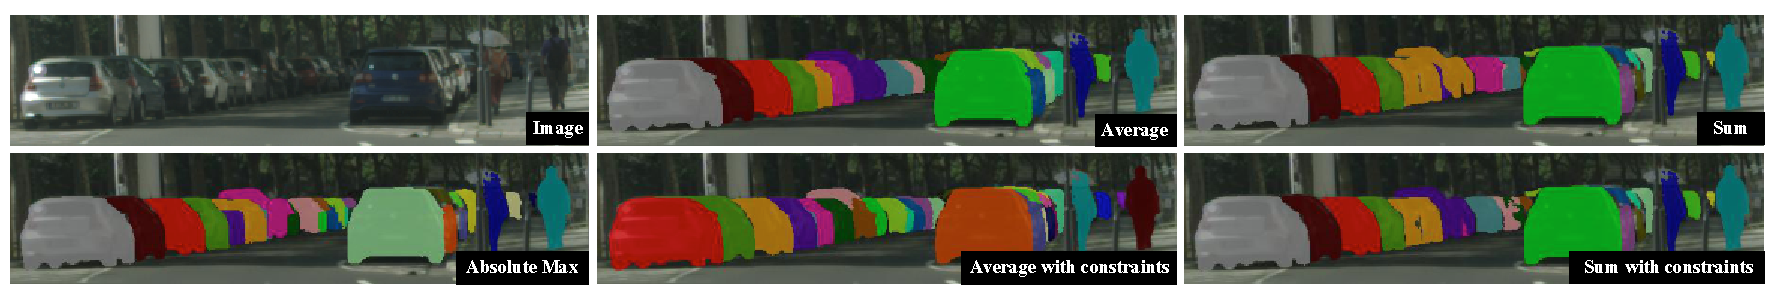
\includegraphics[width=\textwidth]{./figs/cityscapes_compare_4.pdf} % left bottom right top
\caption{Visual results given by different \algname{} linkage criteria on a crop of a CityScapes image}\label{fig:cityscapes}
\end{figure}
